\documentclass{article}
\usepackage{graphicx} % Required for inserting images
\usepackage{geometry}
\usepackage[colorlinks=true, linkcolor=blue, urlcolor=blue]{hyperref}

 \geometry{
 a4paper,
 left=25mm,
 right=25mm,
 top=30mm,
 bottom=30mm
 }

\usepackage[french]{babel}
\usepackage[T1]{fontenc}
\usepackage{lmodern}
\usepackage{hyperref}
\usepackage{wrapfig}

\title{Rapport de projet : Chat201 – édition thread \& réseau}
\author{Daniel DEFOING (\texttt{ddef0003}) \and 
        Belinda ÖZNUR (\texttt{bozn0002}) \and
        Haluk YILMAZ (\texttt{hyil0002})}
\date{\today}

\begin{document}
\pagenumbering{gobble}

\maketitle
\tableofcontents
\newpage

\pagenumbering{arabic}
\section{Introduction}
\noindent Ce rapport décrit globalement la conception du second projet dans le cadre du cours de Systèmes d'Exploitation
(INFO-F201). Il présente les choix de conception qui ont guidé notre développement, et les difficultés qui ont pu survenir durant celui-ci. Pour voir de façon précise les changements ayant eu lieu tout au long du projet et la contribution de chacun, veuillez consulter \href{https://github.com/Daniel-Dfg/OS_Projet_2}{le repository GitHub de notre projet}.

\section{Choix du langage :pourquoi C++ plutôt que C ?}

\subsection*{Des outils qui facilitent le développement en général}
\noindent Une raison fondamentale qui a guidé cette décision est que C++ possède des fonctionnalités absentes en C tels que les références, les chaînes de caractères (ou \textit{strings}, qu'on a souvent subsitués aux \texttt{char*[]}) ou encore les classes.
On peut aussi parler des conteneurs STL comme \texttt{std::vector} ou \texttt{std::queue} \cite{std::queue}, très utilisés dans cette implémentation du projet.


\noindent Or, dans le cadre du projet présenté ici, ces éléments apportent une plus-value non négligeable en permettant de structurer un code de façon plus fine qu'en C ou de simplifier grandement certaines opérations. L'exemple le plus trivial qu'on peut donner de ceci est le passage de paramètres par référence plutôt que par pointeur dans certaines fonctions, qui permet une gestion plus sûre de la mémoire.

\subsection*{Des librairies qui fournissent des abstractions utiles pour ce projet}
\noindent On va illustrer ce point en parlant des \textit{threads}. En langage C, on utilisera \texttt{pthread.h} \cite{pthread.h} pour les gérer, alors qu'en C++ on a par exemple accès à la librairie standard \texttt{std::thread} \cite{std::thread}, qui permet d'abstraire certaines opérations de la librairie en C (par exemple, accéder au thread courant avec \texttt{std::this\_thread} \cite{std::thread}).

\noindent Utiliser C++ permet donc l'usage de certaines librairies standard absentes en C qui permettent d'abstraire des opérations de librairies \textit{correspondantes} en C.

\subsection*{Pas de perte notable à ne pas utiliser le langage C}
\noindent C++ reste évidemment compatible avec C : il n'existe pas d'opération en C infaisable exactement de la même façon en C++ \cite{StackOverflow-C}.
De plus, les deux langages étant connus pour leur rapidité d'exécution, la performance du C++ n'est pas dégradée de façon significative par rapport au C dans le cadre de ce projet. L'utiliser permet donc de tirer parti ses abstractions discutées plus haut (voir 2 sections précédentes) tout en gardant une très bonne efficacité.


\noindent Tout ceci montre que les avantages majeurs ont été trouvés à utiliser C++ plutôt que C, alors qu’aucun avantage n’a été identifié en faveur de l’utilisation de C par rapport à C++. Ce choix du langage s’est donc naturellement imposé comme le plus adapté.

\section{Visualisation de l'architecture du programme}
\noindent Cette section discute des choix de conception du programme final, des considérations qui permettront au lecteur de mieux comprendre la nature de ces choix et des problèmes rencontrés qui en ont suivi.

\subsection{Le serveur en tant que \textit{point relais} des clients}
\noindent La structure d'un programme client-serveur tel que celui présenté ici peut être visualisée très simplement sous la forme d'un Graphe Étoile \cite{Graphe Étoile}, avec le serveur au centre et les clients aux extrémités de chaque branche.
\begin{figure}[ht]
    \centering
    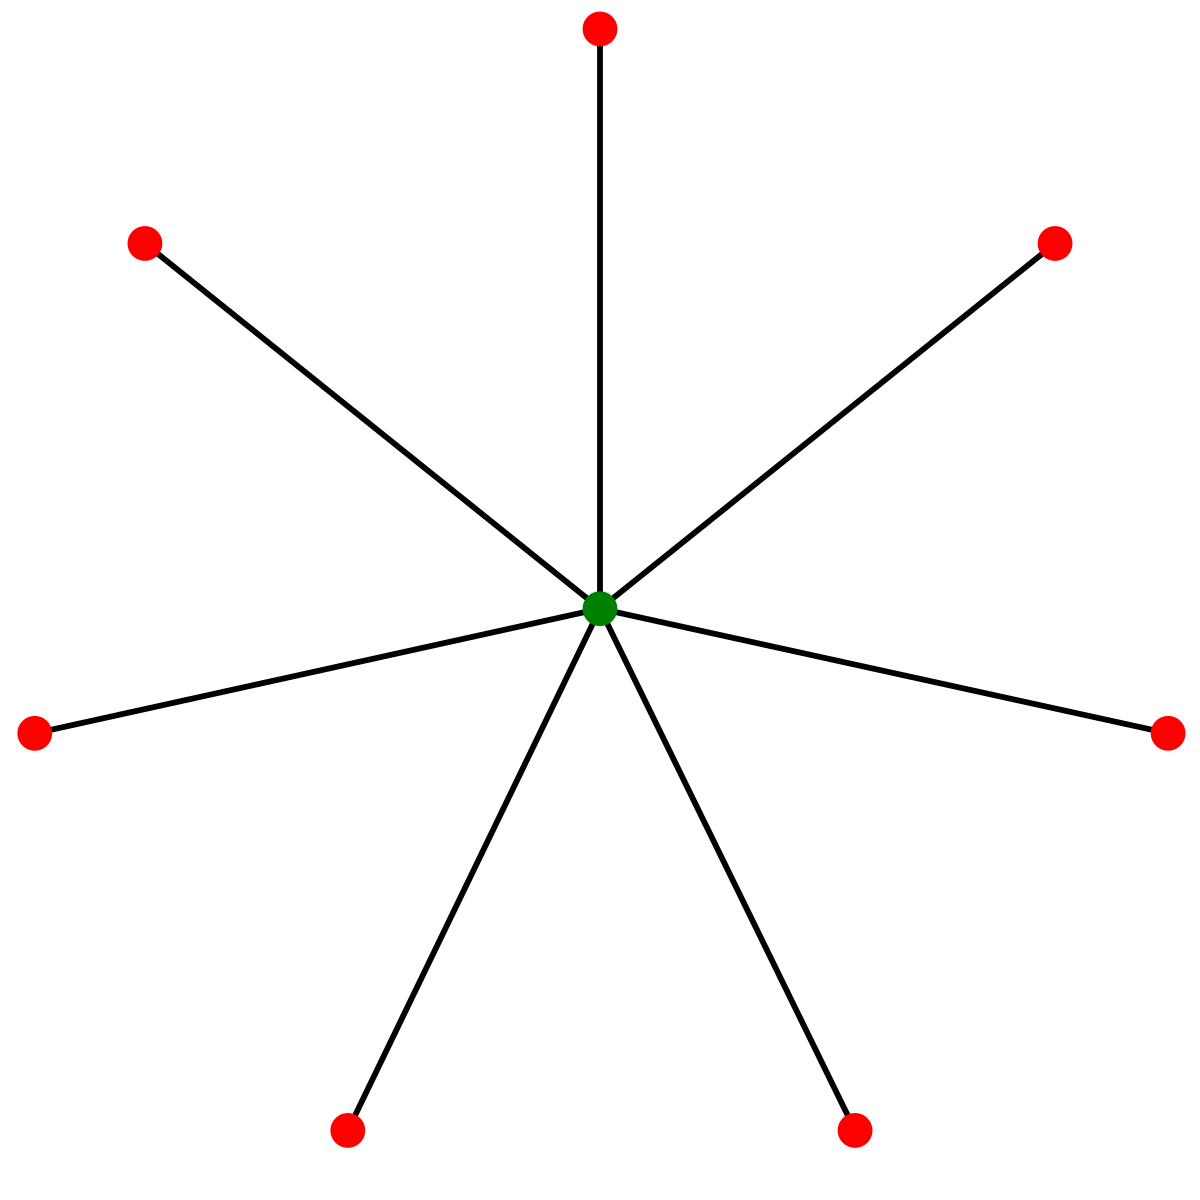
\includegraphics[width=0.2\linewidth]{etoile.png}
    \caption{\textit{Graphe Étoile typique.}}
\end{figure}

\noindent Cette représentation montre bien qu'un seul serveur se charge de \textit{relayer} les informations à passer d'un client à un autre ou d'un client vers lui-même (confirmation de (dé)connexion notamment).

\noindent Dans la suite, on verra en profondeur la façon dont les sommets de ce graphe communiquent.

\subsection{Choix d'implémentation communs aux clients et au serveur}

\subsubsection{Du protocole de communication}
Le choix du \textit{Transmission Control Protocol} \cite{TCP-IP} comme moyen de communication client-serveur n'était pas un "choix" à proprement parler, mais il convient de mentionner que sa mise en place a été faite en suivant globalement la méthode décrite dans la séance de Travaux Pratiques associée \cite{TP_OS}. Pour ce qui est de protocole de réseau, ce sont les adresses de famille IPv4 qui sont utilisés.

\subsubsection{De la méthode d'envoi des messages}
\noindent Il a été décidé d'abstraire l'échange d'informations entre les clients et le serveur principalement par une classe \texttt{Message}. Un point très important qui découle de ce choix d'implémentation est qu'on a utilisé des \texttt{std::string} \cite{std::string} pour garantir une gestion dynamique de la mémoire et simplifier les opérations de manipulation des chaînes de caractère.

\subsection{Conception des clients}

\subsubsection{Capacités d'envoie et de réception}
 Tout client possède un socket pour communiquer avec le server. Ces sockets possèdent 2 buffers par défaut dont l'un pour l'écriture et l'autre pour la lecture. La taille d'un buffer change d'un OS ou d'une machine à l'autre. Cependant ces tailles vont des dizaines à des centaines de Ko. Étant donné que chaque message a au plus 1 Ko et que chaque message est traité très rapidement dés l'envoi ou la réception, ces tailles sont largement suffisants dans le cadre de ce projet. Si toutefois on arrivait à une situation de buffer plein, alors le server se chargera de déconnecter l'utilisateur en question.

Il serait utile de rajouter que la taille par défaut donnée par la machine pour ces buffers de socket IPv4 peut être augmenté. On peut multiplier jusqu'à des dizaines de fois ceux-ci en choisissant la valeur maximale. Nous ne l'avons pas fait dans le cadre de ce projet que les valeurs offertes par défaut sont suffisantes.



\subsubsection{Deux threads, un socket par client}
 La section précédente se focalise sur l'aspect taille du problème. Pour ce qui est de l'aspect temporel dans la gestion de ces 2 buffers, nous utilisons deux threads. Le thread noyau qui est créé en même temps que le processus est dédié à l'envoi de messages (qui doit donc en quelque sorte remplir le buffer des messages à envoyer, puis la vider progressivement) tandis que le second thread créé manuellement est dédié à la réception des messages (qui doit donc vider le buffer et afficher le contenu de messages entrants). Ainsi les deux buffers ne sont pas limités par l'éxécution de l'autre.


 \noindent Cette division du processus client en deux threads est due à des contraintes évidentes de performance et autorise le client à envoyer et recevoir des messages simultanément (gestion asynchrone des communications).



\subsubsection{Gestion de la (dé)connexion au serveur}
\noindent Tout client doit suivre le protocole TCP \cite{TCP-IP} pour initialiser sa connexion et doit s'identifier auprès du serveur. Si le client n'arrive pas à se connecter au server pour une certaine raison, il réenvoie des demandes de connexion périodiquement.
(incomplet)


 Gestion de la déconnexion (quel thread tue l'autre, comment on se déconnecte) TODO :

1. Signalement de déconnexion via un attribut et fermeture des sockets

2. Attente de la fin des opérations en cours

3. Terminaison du thread non-noyau

4. Terminaison du processus

En cas d'erreur, un exit est provoqué avec le code d'erreur correspondant. Ceci ne pose pas de problème car il n'y a pas de ressources à gérer dynamiquement. Les données de l'instance sont supprimés, les sockets sont fermés par le système, les threads sont terminés automatiquement.

\subsection{Conception du serveur}

\subsubsection{De l'utilisation de \texttt{poll}}
\noindent \texttt{poll} \cite{poll} est l'outil qui a été choisi côté serveur pour gérer les connexions et envoi de messages par les clients. Il fonctionne ainsi \cite{poll} :
\begin{enumerate}
    \item Initialiser un \texttt{std::vector} de \texttt{pollfd} (descripteurs de fichier) pour gérer les communications. Chaque entrée dans ce vecteur correspond à une socket connecté au serveur, y compris le socket principal qui gère les nouvelles connexions.
    \item Pour chaque client qui se connecte au serveur, une nouvelle entrée  est ajoutée au \texttt{std::vector}. Symétriquement, ors d'une déconnexion, il faut parcourir ce vecteur pour localiser et supprimer l'entrée correspondante.
    \item \texttt{poll} est \textit{level-triggered}, ce qui signifie que tant qu'un descripteur de fichier est prêt à être traité, l'entrée correspondante dans le vecteur seras signalée. Le serveur est donc "notifié" tant que les données sont disponibles, \cite{LevelEdgeTrigger} \cite{PollTrigger} et il doit se charger de traiter explicitement les évenements signalés pour éviter que ces notifications ne persistent indéfiniment.\\ En pratique, il \textit{boucle} sur le vecteur pendant toute sa durée de vie.
    \item Lorsqu’un événement de lecture est détecté sur une entrée du vecteur, le serveur lis le message du client. Il traite ensuite ce message, vérifie sa validité (taille, format..), puis il recherche à qui le client expéditeur a voulu transmettre son message \footnote{En pratique, on recherche le nom du client récepteur dans un \texttt{std::unordered\_map} avec le nom du client comme clé et son \texttt{pollfd} comme valeur.} et, s'il existe, écrit dans le \texttt{pollfd} du client récepteur.


    Si le destinataire spécifié du message ne fait référence à aucun client connecté, un message d'erreur est renvoyé au client.
    Si le message à envoyer n'est pas dans le bon format, (au minimum 2 mot séparé d'un espace) le serveur ignore la requête.
    Si le message à envoyer est plus grand que 1024 octets, le client n'est pas déconnecté : l'énoncé du projet spécifiait que le client devait être déconnecté \textit{si le serveur \textbf{recevait} un message excédant 1024 octets}, mais notre implémentation \textit{prévient} cette éventualité en n'envoyant tout simplement pas les messages trop massifs. À la place, le client est averti que son message est trop long.
\end{enumerate}


\section{Améliorations non réalisées de l'implémentation actuelle}
\subsection{\texttt{epoll} comme alternative à \texttt{poll}}
\texttt{epoll} \cite{epoll} fonctionne de façon assez similaire à \texttt{poll}, mais a deux différences majeures:
\begin{enumerate}
    \item Il ne fonctionne que sur les systèmes d'exploitation Linux (ou basés sur Linux);
    \item Il peut être \textit{edge-triggered} (une "notification" est envoyée \textit{à l'instant} où des données sont disponibles) ou \textit{level-triggered} (des "notifications" sont envoyées en continu tant que des données sont disponibles). \cite{LevelEdgeTrigger}
    \item On peut aller chercher les données uniquement des \textit{file desciptors} actifs (donc : ceux qui ont reçu un message) plutôt que de devoir itérer sur l'ensemble des \textit{file descriptors} disponibles (ce qui est malheureusement nécessaire pour \texttt{poll}). \cite{EpollTrigger}
\end{enumerate}

\noindent En clair, \texttt{epoll} est cité comme une alternative plus \textit{performante} que \texttt{poll}, mais n'a pas été implémenté dans le cadre de ce projet car l'API est plus complexe à utiliser que celle de \texttt{poll}. L'utilisation d'un mécanisme tel que \texttt{epoll} aurait certainement été indispensable dans le cadre d'un serveur qui devrait accueillir plusieurs milliers d'utilisateurs en simultané ou qui devrait transmettre des données plus volumineuses que du simple texte.

Cependant, l'implémentation d'\texttt{epoll} aurait tout à fait pu être fait en quelques jours supplémentaires.

\subsection{\texttt{boost::asio} comme alternative à \texttt{poll} (réf. nécessaire)}
La première itération du programme visait à utiliser \texttt{boost::asio}, une bibliothèque puissante basée sur \texttt{epoll} qui fournissait une automatisation de certains traitements (comme la mise en place d'un \textit{thread pool} côté serveur par exemple).

\noindent Cependant, nous avons constaté que son utilisation représentait une solution qui dépasse le cadre de ce cours pour un serveur ayant du être réalisé en 2 semaines, ayant du gérer un nombre restreint de connexions simultanées (1000), et traiter des messages contenant uniquement du texte brut. De plus, bien que très instructif, nous n’étions pas assez à l’aise avec tout les aspects et la richesse de cette bibliothèque dans le temps imparti. Cette situation nous a permis d'explorer d’autres solutions, comme \texttt{poll}, qui étaient plus adaptées dans le cadre de ce cours.

\noindent Malgré l'abandon de cette solution, l’utilisation de \texttt{boost::asio} nous a tout de même permis d'approfondir une multitudes de concepts, tels que le fonctionnement et l'optimisation de grand serveurs, les mécanismes asynchrones, \texttt{epoll}.


\subsection{Attente active pour les FIFOs côté client (retirer cette section?)}
\noindent On l'a vu en section 3.3, tout client est séparé en deux threads dont l'un gère une FIFO pour les messages entrants et l'autre les messages sortants. Cependant, l'implémentation actuelle de ce projet fait que le contenu des FIFOs est vérifié en permanence tant que le client est connecté \footnote{On pourrait en quelque sorte parler d'\textit{attente active} de la part du client. \cite{Attente Active} }

\noindent Par manque de temps, un système plus propre n'a pas pu être mis en place, mais on peut en esquisser le fonctionnement théorique (qui aurait certainement pu, comme pour \texttt{epoll}, être implémenté en quelques jours) :
\begin{enumerate}
    \item Initialement, la FIFO des messages entrants est vide. Dès qu'un message est envoyé au client, celui-ci est notifié et \texttt{pop()} un élément de la FIFO pour le traiter.
    \item Chaque nouveau message entrant correspond à une nouvelle "notification" pour le client, à une nouvelle tâche à faire : on peut donc facilement avoir un "compteur de tâches à faire" qui indique combien de fois le client doit extraire un message de la FIFO. Ce compteur serait naturellement décrémenté dès que le client aurait fini une tâche.

    Par exemple, si un client reçoit 3 messages en même temps, il est censé être notifié 3 fois et donc \texttt{pop()} le premier élément de la FIFO 3 fois (ce qui vide exactement la FIFO, en principe).
    \item Lorsque la FIFO est vide, le client a donc en théorie réalisé toutes les tâches qui lui étaient assignées et n'a par conséquent pas besoin de vérifier son contenu en permanence.
\end{enumerate}

\section{Difficultés rencontrées et solutions trouvées}
\subsection{Problèmes de synchronisation côté serveur}
Pendant le développement, l'hypothèse selon laquelle on aurait pu faire face à des problèmes de synchronisation côté serveur (typiquement, en recevant deux messages en même temps) était bien présente.

Cependant, dans l'implémentation actuelle, on peut écarter cette possibilité puisque le serveur traite les événements de manière séquentielle, en \textit{mono-thread} grâce à \texttt{poll}, éliminant ainsi à la fois les risques d'accès concurrents et à la fois les problèmes d'ordre d'envoi et réception des messages \footnote{Comprenez : si 3 messages A, B, C sont lus dans cet ordre, alors ils seront aussi envoyés dans l'ordre A, B, C.}. Chaque événement est ainsi traité de manière séquentielle.

\subsection{Asynchronie des signaux}
Le programme présenté ici gère les signaux \texttt{SIGINT} et \texttt{SIGPIPE}. Les signaux étant asynchrones, une difficulté de ce projet était de les gérer pour :
\begin{itemize}
    \item Éviter l'interruption inopinée d'opérations cruciales (écriture/lecture notamment)
    \item Permettre de définir les actions à exécuter en cas de réception d'un signal
    \item Garantir une \textit{communication} adéquate entre les clients et le serveur (lorsqu'un client se déconnecte, il doit pouvoir le communiquer au serveur pour que celui-ci évite de relayer des messages dans le vide)
\end{itemize}

Il a donc été décidé de centraliser la gestion des signaux dans une classe dédiée, \texttt{SignalManager}, pour laquelle on peut lister ses choix de conception les plus importants.



\subsubsection{Différence entre le mode normal et le mode \texttt{manuel}}
Lors de l'arrêt du programme, le signal manager prend en compte l'absence (\texttt{SignalManager::signalHandler}) ou la présence du mode \texttt{manuel} (\texttt{SignalManager::signalHandlerManuel}).

\subsubsection*{Masquage des signaux pour le thread récepteur côté client}
 On en a déjà discuté dans ce rapport, mais tout client possède deux threads distincts, un pour l'envoi et un autre pour la réception de messages. Ce dernier possède un \textit{masque} qui fait qu'il ignore tous les signaux qui lui parviennent. Ce choix a été fait pour centraliser la gestion des signaux côté client dans le thread principal.

\subsubsection*{Communication de signaux entre threads}
Le masquage des signaux était une solution à la répartition des gestions des signaux par les threads. Mais il est également possible d'envoyer des signaux entre les threads. Ceci est possible car chaque thread possède un ID. Si le second thread qui s'occupe de la lecture via le server reçoit un signal qui indique que le serveur nous a déconnecté alors il est possible de prévenir le thread noyau pour qu'il s'occupe du reste via un pthread\_kill().



\subsection{Situations de concurrence}
Etant donné que deux threads sont utilisés dans le cadre de ce projet, il était nécessaire de gérer explicitement les accès cas de concurrence pour :
\begin{itemize}
    \item L'affichage des messages envoyés ou reçu sur le terminal.
    \item La modification de la mémoire pour y ajouter ou retirer des messages.
\end{itemize}
Ceci a été réalisé grâce à l'utilisation d'un mutex différent pour chaque cas.

\subsubsection*{Deadlocks}
Dans le cadre de ce projet, diverses situations de deadlocks/d'interblocages ont également fait surface. Il a donc fallu utiliser les threads et les mutex d'une façon réflechie pour éviter cela. Voici deux cas qu'il a fallu gérer/corriger:
\begin{itemize}
    \item L'appel d'un méthode qui sert à déconnecter le client par le second thread. Ceci pose problème car la méthode responsable de la déconnexion essaye de joindre ce même thread pour le terminer. Il faut donc éviter d'appeler cette méthode par ce thread et seulement y faire appel par le thread noyau.
    \item Le blocage d'un mutex avant l'appel d'une autre méthode qui utilise lui même ce mutex dans le même scope. Ceci provoque un interblocage car quand la méthode est appelé et qu'il veut opérer il doit attendre que le mutex soit libéré indéfiniment.
\end{itemize}



\subsection{Garantie de l'intégrité du contenu partagé par les clients}

\subsubsection{Gestion des tailles limites}

Pour garantir l'intégrité du contenu partagé par les clients, nous avons imposé des limites strictes sur la taille des pseudos (maximum de 30 octets) et des messages (maximum de 1024 octets) à la fois coté client et coté serveur. En cas de dépassement de la taille du message, et que ce message parviens coté serveur malgré la protection coté client, le message est rejeté et le serveur déconnecte le client.

\subsubsection{Fiabilité de la transmission des messages}

Malgré toutes les précautions prises pour avoir un programme \textit{safe}, il est toujours possible qu'on rencontre des cas où le client rencontre des erreurs (à cause d'un matériel défectueux, par exemple).

Ce cas d'erreur \textit{externe, indéfinie} est également géré par notre programme (du moins en partie) : si un problème de ce type est détecté, le client problématique est déconnecté et si un autre client essayait de lui envoyer des messages (qui n'arrivaient pas à destination à cause de ces fameux problèmes \textit{indéfinis}, justement), il est notifié du problème.

\begin{thebibliography}{999}
    \bibitem{std::queue}
    \texttt{std::queue} - cppreference (dernière modification : 2024, 2 août)

    URL : \url{https://en.cppreference.com/w/cpp/container/queue}

    \bibitem{pthread.h}
        pthreads(7) — Linux manual page (dernière modification : 2024, 15 juin).

        URL : \url{https://www.man7.org/linux/man-pages/man7/pthreads.7.html}

    \bibitem{std::thread}
        \texttt{std::thread} - cppreference (dernière modification : 2023, 24 octobre).

        URL : \url{https://en.cppreference.com/w/cpp/thread/thread}

    \bibitem{StackOverflow-C}
        StackOverflow - \textit{Is there anything that can be done in C and not in C++ and the opposite way ? [closed]} (dernière modification : 2010, 9 décembre)

    URL : \url{https://stackoverflow.com/questions/4403328/is-there-anything-that-can-be-done-in-c-and-not-in-c-and-the-opposite-way}

	\bibitem{Graphe Étoile}
		Wikipedia : \textit{Graphe étoile} (dernière modification : 2019, 21 janvier)

        URL: \url{https://fr.wikipedia.org/wiki/Graphe_%C3%A9toile}

    \bibitem{TCP-IP}
    Wikipedia : \textit{Transmission Control Protocol} (dernière modification : 2024, 17 décembre)

    URL : \url{https://en.wikipedia.org/wiki/Transmission_Control_Protocol}

    \bibitem{TP_OS}
    GOOSENS J., MARKOWITCH O., cours de \textit{Systèmes d'Exploitation} (ULB), TP n°6 : Programmation réseau

    \bibitem{std::string}
    C++ Programming Language : \texttt{std::string} (dernière modification : inconnu)

    URL : \url{https://cpp-lang.net/docs/std/containers/strings/string/}

    \bibitem{std::mutex}
    \texttt{std::mutex} - cppreference (dernière modification : 2024, 6 mars)

    URL : \url{https://en.cppreference.com/w/cpp/thread/mutex}

    \bibitem{poll}
    poll(2) - Linux manual page (dernière modification : 2024, 15 juin).

    URL : \url{https://www.man7.org/linux/man-pages/man2/poll.2.html}


    \bibitem{LevelEdgeTrigger}
    StackOverflow - \textit{Level vs Edge Trigger Network Event Mechanisms} (dernière modification : 2022, 28 août).

    URL : \url{https://stackoverflow.com/questions/1966863/level-vs-edge-trigger-network-event-mechanisms}

    \bibitem{PollTrigger}
    StackOverflow - \textit{Is poll() an edge triggered function?} (dernière modification : 2013, 25 février).

    URL : \url{https://stackoverflow.com/questions/15072165/is-poll-an-edge-triggered-function?rq=3}

    \bibitem{epoll}
    epoll(7) — Linux manual page (dernière modification : 2024, 12 juin).

    URL : \url{https://www.man7.org/linux/man-pages/man7/epoll.7.html}

    \bibitem{EpollTrigger}
    StackOverflow - \textit{What is the purpose of epoll's edge triggered option?} (dernière modification : 2022, 25 septembre).

    URL : \url{https://stackoverflow.com/questions/9162712/what-is-the-purpose-of-epolls-edge-triggered-option?rq=3}

    \bibitem{Attente Active}
    Wikipedia : \textit{Busy Waiting} (dernière modification : 2024, 2 novembre).

    URL : \url{https://en.wikipedia.org/wiki/Busy_waiting}
\end{thebibliography}
Toutes sources consultées pour la dernière fois le 21/12/24, 16h.

\end{document}

